\documentclass{beamer}
\setbeamertemplate{navigation symbols}{}

\addtobeamertemplate{navigation symbols}{}{%
	\usebeamerfont{footline}%
	\usebeamercolor[fg]{footline}%
	\hspace{1em}%
	\insertframenumber/\inserttotalframenumber
}
\usepackage[utf8]{inputenc} % allow utf-8 input
\usepackage[T1]{fontenc}    % use 8-bit T1 fonts
\usepackage{hyperref}       % hyperlinks
\usepackage{url}            % simple URL typesetting
\usepackage{booktabs}       % professional-quality tables
\usepackage{amsfonts}       % blackboard math symbols
\usepackage{nicefrac}       % compact symbols for 1/2, etc.
\usepackage{microtype}      % microtypography
\usepackage{xcolor}         % colors
\usepackage{setspace}
\usepackage{url}
\usepackage{amssymb}
\usepackage{amsmath}
\usepackage{amsthm}
\usepackage{graphicx}
\usepackage{amsmath}
\usepackage{hyperref}   % Package for hyperlinks
\usepackage{tikz}
%\usepackage{enumitem}
\usepackage{stackengine,scalerel}

\newcommand\overstarbf[1]{\ThisStyle{\ensurestackMath{%
			\stackengine{0pt}{\SavedStyle\mathbf{#1}}{\smash{\SavedStyle*}}{O}{c}{F}{T}{S}}}}
\newcommand\overstar[1]{\ThisStyle{\ensurestackMath{%
			\setbox0=\hbox{$\SavedStyle#1$}%
			\stackengine{0pt}{\copy0}{\kern.2\ht0\smash{\SavedStyle*}}{O}{c}{F}{T}{S}}}}

\newcommand*{\wackyenum}[1]{%
	\expandafter\@wackyenum\csname c@#1\endcsname%
}

\renewcommand{\t}{\mathbf{t}}
\newcommand{\x}{\mathbf{x}}

\usepackage{bbm}
\DeclareMathOperator*{\argmax}{arg\,max}
\DeclareMathOperator*{\argmin}{arg\,min}
%\newcommand{\indep}{\perp \!\!\! \perp}
\newcommand\indep{\protect\mathpalette{\protect\independenT}{\perp}}


\def\independenT#1#2{\mathrel{\rlap{$#1#2$}\mkern2mu{#1#2}}}
\newtheorem{proposition}{Proposition}
\newtheorem{defn}{Definition}
\newtheorem{assump}{Assumption}
\newtheorem{cond}{Condition}

\DeclareMathOperator*{\E}{\mathbb{E}}
\DeclareMathOperator*{\Var}{\text{Var}}
\DeclareRobustCommand{\firstsecond}[2]{#2}
\usepackage[capposition=top]{floatrow}

\usetikzlibrary{shapes,arrows}

\newcommand{\maxt}{\mathcal{T}_q^\text{Max}}
\newcommand{\mint}{\mathcal{T}_q^\text{Min}}
\newcommand{\sstar}{\overstar{\mathcal{S}}}


\newcommand{\maxthat}{\hat{\mathcal{T}}_q^{\text{Max}(b)}}
\newcommand{\minthat}{\hat{\mathcal{T}}_q^{\text{Min}(b)}}
\newcommand{\tautrue}{\tau(\tprime, \tprime')}


\newcommand{\maxp}{p_i^{\text{Max}}}
\newcommand{\minp}{p_i^{\text{Min}}}

\newcommand{\maxw}{w^\text{Max}}
\newcommand{\minw}{w^\text{Min}}

\newcommand{\cov}{\text{Cov}}
\newcommand{\phat}{\hat{p}}


\newcommand{\tq}{\mathcal{T}_q}
\newcommand{\tprime}{\mathcal{T}'}
\newcommand{\tstar}{\mathcal{T}^*}
\newcommand{\tstarstar}{\mathcal{T}^{**}}

\newcommand{\maxphat}{\hat{p}^\text{Max}}
\newcommand{\minphat}{\hat{p}^\text{Min}}


\newcommand{\baseprob}{\hat{P}(\mathcal{T}'=\maxt \cap \mathcal{T}''=\mint)}
\newcommand{\baseprobn}{\hat{P}^{(n)}(\mathcal{T}'=\maxt \cap \mathcal{T}''=\mint)}

\newcommand{\tauhat}{\hat{\tau}(\tprime, \tprime')}
\newcommand{\tauhatn}{\hat{\tau}^{(n)}(\tprime, \tprime')}
\newcommand{\baseprobstar}{\hat{P}(\tstar=\maxt \cap \tstarstar=\mint)}
\newcommand{\tauhatstar}{\hat{\tau}(\tstar, \tstarstar)}


\newcommand{\maxtb}{\mathcal{T}_q^{\text{Max}(b)}}
\newcommand{\mintb}{\mathcal{T}_q^{\text{Min}(b)}}


\newcommand{\sminusk}{\mathcal{S}_{-k}}
\newcommand{\sk}{\mathcal{S}_{k}}
\newcommand{\sest}{\mathcal{S}^{\text{Est}}}
\newcommand{\ssplit}{\mathcal{S}^{\text{Prob}}}
\newcommand{\var}{\text{Var}}
\newcommand{\mcseq}{\text{MCSE}_q}

\newcommand{\ind}{\mathbbm{1}}
\usepackage{appendix}

\begin{document}
	\title{Survey Weighting}
	\author{Zach Markovich}
	%%% Title
	\frame[plain]{\titlepage}
	\setcounter{framenumber}{0}

\begin{frame}{Why Weight?}
\begin{itemize} 
\item Suppose there's a population: $Y_1 \dots Y_N$ \pause 

\item So you sample a subset of them, uniformly at random, and ask their opinion \pause 

\item If $D_i$ is a dummy variable indicating whether unit $i$ was sampled, then the simple mean of your sample is an unbiased estimator for the true mean:\pause 

$$
\E\left(\sum_{i=1}^N \frac{D_i Y_i}{\sum_{i=1}^N D_i}\right) = \E\left(\sum_{i=1}^N \frac{Y_i}{N}\right) 
$$	

\pause 
\item Unfortunately, in the real world we don't get a true random sample \pause 
\item Specifically, if some variable influences both $P(D_i=1)$ and $Y_i$, the simple mean will be a biased estimator
\end{itemize}
\end{frame}

\begin{frame}{Declining response rates have intensified this problem}
	\centering 
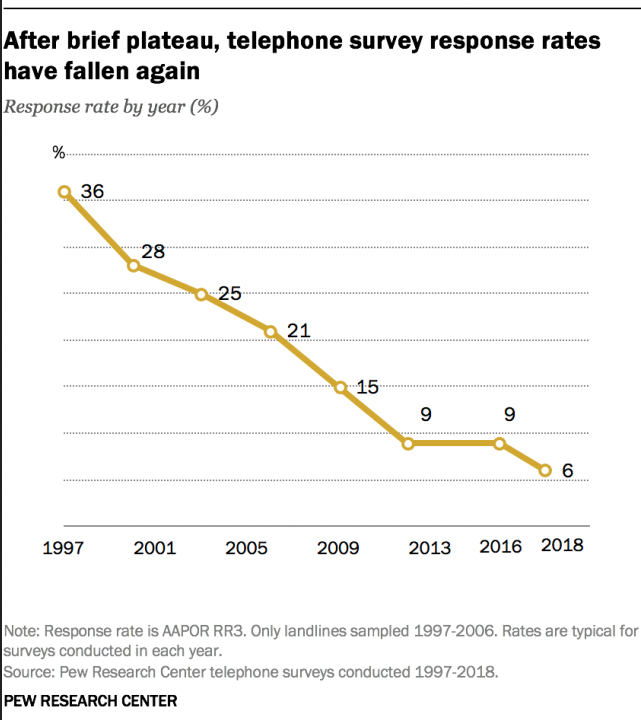
\includegraphics[height=.9\textheight]{response_rates.png}
\end{frame}


\begin{frame}{Quota Sampling}
	\begin{itemize}
		\item Declining response rates have led many survey researchers to abandon random (or probability) sampling entirely \pause 
		\item Instead, they've turned to online panels -- sometimes they will require the sample conform to some demographic quotas (quota sampling) -- this can reduce the need for weights \pause 
		\item Other times, you're just stuck with what there is (i.e. MTurk) \pause 
		\item The same general idea applies -- want to draw conclusions about a population that's different from our sample
	\end{itemize}
\end{frame}


\begin{frame}{Weighting to the rescue}
In an ideal world, we'd know the true probability that a unit was sampled from the population: $P_i = P(D_i = 1)$. Then:

$$
\E\left(\sum_{i=1}^N \frac{P_i^{-1} Y_i}{\sum_{i=1}^N P_i^{-1}}\right) = \E\left(\sum_{i=1}^N \frac{Y_i}{N}\right) 
$$

Of course, in the real world, we don't actually know the weights, so instead we guess
\end{frame}


\begin{frame}{Designing Survey Weights}
	\begin{itemize} 
		\item Observe a random sample drawn from the \textit{sample frame} with known probabilities \pause 
		\item Wish to use the sample to draw inferences about a different population \pause 
		\item Specifically, will use covariates with a known frequency in the target population to produce estimates that will be representative of the target population

	\end{itemize}
\end{frame}



\begin{frame}{Post-Stratification}
\begin{itemize} 
\item Most common and straightforward approach to weighting \pause 
\item Assumes that for some set of demographic covariates, $X_1 \dots X_N$ %with support $\mathcal{X}$, we know 
%$P(X_i=x)$ for all $x \in \mathcal{X}$. Then,

$$
w_i = \frac{P(X_i \text{ in Population})}{P(X_i \text{ in Sample Frame})} P(\text{i drawn from sample frame})
$$

Note, often use value of $P(X_i \text{ in Sample Frame})$ estimated from the sample. \pause Then estimate mean as, \pause 

$$
\frac{\sum_{i =1}^N w_i Y_i}{\sum_{i=1}^N w_i}
$$

\end{itemize}
\end{frame}


\begin{frame}{Multi-level Regression and Post-stratificiation (MrP)}
	\begin{itemize} 
		\item It is common to replace $Y_i$ in the post-stratification estimator with the predictions from a hierarchical model \pause 
		\item The estimator then becomes: 		
		
		$$
		\frac{\sum_{i =1}^N w_i \widehat{\E\left(Y_i|X_i \right)} }{\sum_{i=1}^N w_i}
		$$
		
		Which simplifies to:

		$$
		\sum_{x \in \mathcal{X}} P(X_i=x \text{ in population}) \widehat{\E\left(Y_i|X_i=x \right)}
			$$

		\pause 
		\item There are two advantages of this:
		
		\begin{itemize}
			\item Allows us to make predictions about $\widehat{\E\left(Y_i|X_i=x \right)}$ for empty cells
			\item Bayesian methods regularize estimates for $\widehat{\E\left(Y_i|X_i=x \right)}$ for small cells
		\end{itemize}
		
	\end{itemize}
\end{frame}


\begin{frame}{Raking}
	\begin{itemize} 
		\item Very often, we don't have knowledge of the joint frequency of all demographic traits\pause 
		\item Instead we might just have the marginal means \pause 
		\item \textit{Raking} is a procedure to produce weights will match the population marginal means, while maintaining the sample joint distribution \pause
		\item There are many variations of the exact raking procedure, but they generally involve iteratively balancing the the marginal distribution of each variable
	\end{itemize}
\end{frame}


\begin{frame}{Weight Trimming}
	\begin{itemize}
		\item Sometimes we'll end up with very extreme weights for rare combinations of covariates \pause 
		\item In this case, such extreme weights may lead to an increase in the variance of their estimates that is out of step with the reduction in bias they facilitate \pause 
		\item The only common solution here is to ``trim'' the weights by setting all weights greater than some value to a fixed level\pause 
		\item This level is usually chosen in an ad hoc way (e.g. mak esure no weights are greater than a 10 or a 100)\pause 
		\item More principled techniques exist, but they're not frequently used
	\end{itemize}
\end{frame}


\begin{frame}{Go Over Code}
\end{frame}



\begin{frame}{Choosing the Target Population}
\begin{itemize} 
	\item Sometimes we know the full target population -- say we're working with census data\pause 
	\item Often, the population target is an estimated quantity as well:\pause 
	\begin{itemize}
		\item Might have to interpolate quantities that are only observed at infrequent time intervals (e.g. deciennial census)\pause 
		\item Might impute joint distribution for some variable -- e.g. ecological inference\pause 
	\end{itemize}
	\item Generally, we treat weights as known constants, but this isn't right if the weights are modeled. Bayesian or bootstrap procedures will be the best way to incorporate this into variance estimates, although this isn't often done in practice\pause 
\end{itemize}
\end{frame}


\begin{frame}{Choosing Variables to Weight With}
	\begin{itemize} 
		\item Often there are more available covariates than we can practically use\pause 
		\item This represents a bias-variance tradeoff -- basing weights on more variables reduces bias, but leads to more extreme cells which inflate the variance of the estimate \pause 
		\item A variable that is important to weight with will be a strong predictor of both the \textit{response} and the \textit{sampling probability}\pause 
		\item Weight with a variable that is only related to the sampling probability, but not the outcome will inflate the variance, but not lead to bias\pause 
		\item There are formal methods for optimizing this choice (e.g Caughey and Hartman), but we won't get into them now \pause 
	\end{itemize}
\end{frame}




\begin{frame}{Conclusion}
\begin{itemize}
	\item Survey weighting is about designing weights so that estimates generated from the sample will conform to those generated for some target population\pause 
	\item The two most common approaches to generating these weights are post-stratification and raking\pause 
	\item Both techniques assume that the researcher knows some feature of the target population -- this is not true in practice\pause 
	\item Researchers should focus weighting on variables that are likely to influence both the outcome and the sampling probability \pause 
	\item This is a very active area of methodological research -- the number covariates available for weighting has increased while samples have become increasingly less representative\pause 
	\item Nonetheless, these basic principles will be sufficient for designing weights for most applied projects.
\end{itemize}

\end{frame}




\end{document}